In thes section we will  be showing results for  different aspects of this project this  will  include the following:
\begin{enumerate}
    \item Recorded data from sensors
    \item Recorded data from transciver
    \item Recorded data from  testing the mesh network
\end{enumerate}
\section{Recorded data from sensors}
in this section  will have  tables from the following componets:
\begin{enumerate}
    \item DHT22 \textbf{heat and temp}
    \item AS312 \textbf{Motion }
    \item DFR0026 \textbf{Light}
    \item Raspberry Pi VR 220 \textbf{Camera}
\end{enumerate}
\subsection{DHT22}
\subsubsection{Results during protypeing}
\begin{table}[h!]
    \begin{tabular}{|c|c|c|}
        \hline
        date/time of record & Tempeature &Humidity \\
        \hline\hline
        2024-02-21 00:03:56&22& 66 \\
    \end{tabular}
    \caption{Recorded data from  DHT22 on the \today}
    \label{Recorded data from  DHT22 on the \today}
\end{table}

last we tested if our code  satisfies our  python code after testing the unit test code we upadated see the foolwing message
\begin{figure}[h!]
    \centering
    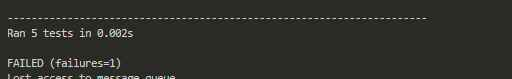
\includegraphics[width=0.5\linewidth]{Images/unit_testoutput.jpg}
    \caption{unit test message for DHT22 module}
    \label{unit test message for DHT22 module}
\end{figure}
\newpage
\subsection{AS312}
\subsubsection{Results during protype}
\begin{table}[h!]
    \centering
    \begin{tabular}{|c|c|}
        \hline
        date/time of record & motion detected(yes/no)\\
        \hline \hline
    \end{tabular}
    \caption{Recorded data from  AS312 on the \today}
    \label{Recorded data from  AS312 on the \today}
\end{table}
\subsection{DFR0026}
\subsubsection{Results during protypes}
for our first test we got  the following  table 
\begin{table}[h!]
    \centering
    \begin{tabular}{|c|c|}
        \hline
        Date/time of record & lux vaules\\
        \hline \hline
    \end{tabular}
    \caption{Recorded data from DFR0026 on the \today}
    \label{Recorded data from DFR0026 on the \today}
\end{table}
\subsection{Raspberry Pi VR 220}
When testing  the Raspberry Pi VR 220
\subsubsection{Results during testing}
\begin{figure}
    \centering
    \includegraphics[options]{name}
    \caption{A photo from \today }
    \label{A photo from \today}
\end{figure}

\section{Recorded data from transciver}
\section{Recorded data from mesh network}